\documentclass[12pt]{scrartcl}
\usepackage{graphicx}
\usepackage{color}
\usepackage{url}
\usepackage{xcolor}
\usepackage{listings}
\usepackage{nameref}
\usepackage[headsepline,footsepline]{scrlayer-scrpage}
\usepackage{biblatex}
\usepackage{float}


\definecolor{mGreen}{rgb}{0,0.6,0}
\definecolor{mGray}{rgb}{0.5,0.5,0.5}
\definecolor{mPurple}{rgb}{0.58,0,0.82}
\definecolor{backgroundColour}{rgb}{0.95,0.95,0.95} %{cmyk}{0.05,0.05,0.05,0.05}

\lstdefinestyle{CStyle}{
    backgroundcolor=\color{backgroundColour},   
    commentstyle=\color{mGreen},
    keywordstyle=\color{blue},
    numberstyle=\tiny\color{mGray},
    stringstyle=\color{mPurple},
    basicstyle=\footnotesize,
    breakatwhitespace=false,         
    breaklines=true,                 
    captionpos=b,                    
    keepspaces=true,                 
    numbers=left,                    
    numbersep=5pt,                  
    showspaces=false,                
    showstringspaces=false,
    showtabs=false,                  
    tabsize=2,
    language=C++
}

\lstdefinestyle{Terminal}{
    backgroundcolor=\color{backgroundColour},   
    commentstyle=\color{black},
    keywordstyle=\color{black},
    numberstyle=\tiny\color{black},
    stringstyle=\color{black},
    basicstyle=\footnotesize,
    breakatwhitespace=false,         
    breaklines=true,                 
    captionpos=b,                    
    keepspaces=true,                 
    numbers=none,                    
    numbersep=5pt,                  
    showspaces=false,                
    showstringspaces=false,
    showtabs=false,                  
    tabsize=2,
}


\pagestyle{scrheadings}
\clearscrheadfoot
%\cfoot{Tobias Gruber}
\cfoot{\pagemark}
\chead{\headmark}
\automark[subsection]{section}


\begin{document}


\begin{titlepage}
    \vfill
	\centering
	{\scshape\LARGE Hochschule München \par}
    {\scshape\Large Fakultät für Informatik \par}
	\vspace{1.5cm}

    


    \vfill
	{\LARGE\bfseries Computational Geometry\\~\\ \par}
	{\LARGE\bfseries Praktikumsaufgabe 1\par}
	\vfill
    \vfill


    \begin{tabular}{ll}
    \normalsize
    Team:  & Christopher Hinz, Tobias Gruber\\
    \end{tabular}

	\vfill

\end{titlepage}

\newpage



\raggedright


\section{Aufgabenstellung}
In dem Tar-File 'strecken.tgz' (s.u.) befinden sich Dateien mit jeweils 4 Koordinaten pro Zeile. 
Diese stellen jeweils die x- und y-Koordinaten eines Start- bzw. Endpunkts einer Strecke dar. 
Lesen Sie jeweils eine Datei ein und ermitteln Sie die Anzahl der sich schneidenden 
(d.h. mindestens ein gemeinsamer Punkt) Strecken, indem Sie jedes Paar von Strecken gegeneinander testen. 
Messen Sie die pro Datei aufgewendete Zeit. Begründen Sie nachvollziehbar, warum die Anzahl der von Ihrem Programm 
jeweils gefundenen Schnittpunkte korrekt ist.

\section{Vorüberlegung}

Um einschätzen zu können inwiefern die Ergebnisse sinnvoll sind sollen an dieser Stelle einige Vorüberlegungen getroffen werden.\\~\\
Welche Anzahl an Schnitten sind zu erwarten bzw. in welchem Wertebereich sollten sich die Ergebnisse bewegen?\\
Die minimal zu erwartende Anzahl an Schnitten wäre für 1.000, 10.0000 und 100.000 Strecken jeweils null. 
Dies ist somit die untere Grenze des zu erwartenden Wertebereichs. 
Die maximale Anzahl an Schnitten würden in dem Fall auftreten, dass sich alle Strecken gegenseitig schneiden. 
Dann wäre nämlich für jede Strecke ein Schnittpunkt mit allen anderen Strecken gegeben.
Damit wären für 1.000 Strecken maximal $1.000*999 = 999.000$ (für 10.000 maximal $10.000*9.999 = 99.990.000$, 
für 100.000 maximal $100.000*99.999 = 9.999.900.000$) zu erwarten.
Dies ist somit die obere Grenze des zu erwartenden Wertebereichs. 


\section{Umsetzung}

\subsection{Programm zur Aufgabenstellung}

\begin{lstlisting}[style=CStyle, caption={p1\_lib.h: Bibliotheksfunktionen},captionpos=b]
#include <fstream>
#include <iostream>
#include <string>
#include <vector>


struct point{
    double x;
    double y;
};

struct line{
    point p1;
    point p2;
};

void read_dat(char* filename, std::vector<line>& target){
    line temp;
    std::ifstream file;
    file.open(filename);
    double k1, k2, k3, k4;
    if(!file.is_open()){
        std::cout << "Could not open file\n";
    }
    while(file >> k1 >> k2 >> k3 >> k4){
        temp.p1.x = k1;
        temp.p1.y = k2;
        temp.p2.x = k3;
        temp.p2.y = k4;
        target.push_back(temp);
    }
    file.close();
}

double ccw(point p, point q, point r){
    double res = (p.x*q.y - p.y*q.x)+ (q.x*r.y - q.y*r.x) + (p.y*r.x  - p.x*r.y);
    return res;
}

bool line_intersect_check(line l1, line l2){
    bool retval = false;
    double ccw_res1 = ccw(l1.p1, l1.p2, l2.p1) * ccw(l1.p1, l1.p2, l2.p2);
    double ccw_res2 = ccw(l2.p1, l2.p2, l1.p1) * ccw(l2.p1, l2.p2, l1.p2);
    if(ccw_res1 <= 0.0 && ccw_res2 <= 0.0){
        retval = true;
        if(ccw_res1 == 0.0 && ccw_res2 == 0.0){
            double lambda1 = (l2.p1.x-l1.p1.x)/(l1.p2.x-l1.p1.x);
            double lambda2 = (l2.p2.x-l1.p1.x)/(l1.p2.x-l1.p1.x);
            if ((lambda1 < 0.0 || lambda1 > 1.0) && (lambda2 < 0.0 || lambda2 > 1.0)) 
                retval = false;
        }
    }
    return retval;
}
\end{lstlisting}



\begin{lstlisting}[style=CStyle, caption={strecken.cpp: Aufgruf der Bibliotheksfunktionen},captionpos=b]
#include "p1_lib.h"
#include <chrono>

int main(){
    auto start = std::chrono::steady_clock::now();


    std::vector<line> lines_vec;
    read_dat((char*)"../strecken/s_1000_1.dat", lines_vec);


    int intersect_counter = 0;
    for(unsigned int i = 0; i < lines_vec.size(); ++i){
        for(unsigned int j = i; j < lines_vec.size(); ++j){
            if(i!=j){
                if(line_intersect_check(lines_vec[i], lines_vec[j])){
                    ++intersect_counter;
                }
            }
        }
    }
    std::cout << "Strecken insgesamt: " << lines_vec.size() << "\n" << "Schnitte zweier Strecken: " << intersect_counter << "\n";

    auto end = std::chrono::steady_clock::now();     
    std::cout << "Runtime: " 
    << (double)std::chrono::duration_cast<std::chrono::microseconds>(end - start).count()/1000 
        + std::chrono::duration_cast<std::chrono::milliseconds>(end - start).count() << " ms\n";

    return 0;
}
\end{lstlisting}

Wie unten zu erkennen ist liegt die Anzahl der Schnitte für alle Fälle (1.000, 10.000, 100.000) im zu erwartenden Wertebereich.
Schnittpunkte:    
\begin{itemize}
    \item 1.000 Strecken: $0<= 62.250 <= 999.000$
    \item 10.000 Strecken: $0<= 6.247.500 <= 99.990.000$
    \item 100.000 Strecken: $0<= 624.975.000 <= 9.999.900.000$
\end{itemize}


\begin{lstlisting}[style=Terminal, caption={testing.cpp: Ausgabe Konsole},captionpos=b]
# s_1000_1.dat
Strecken insgesamt: 1000
Schnitte zweier Strecken: 62250
Runtime: 14.408 ms
#s_10000_1.dat
Strecken insgesamt: 10000
Schnitte zweier Strecken: 6247500
Runtime: 580.073 ms
#s_100000_1.dat
Strecken insgesamt: 100000
Schnitte zweier Strecken: 624975000
Runtime: 55100.2 ms
\end{lstlisting}


\subsection{Programm zum Testen der Funktion}
Neben den getroffenen Vorüberlegungen soll das Programm zusätzlich mit einigen definierten Testfällen validiert werden.
Zum Sicherstellen der korrekten Funktion des Programms sollen verschiedene Streckenanordnungen getestet werden.
Zum Veranschaulichen der getesteten Strecken dient das nachfolgende Bild.\\

\begin{figure}[ht]
    \graphicspath{ {./pictures/} }
    \centering
    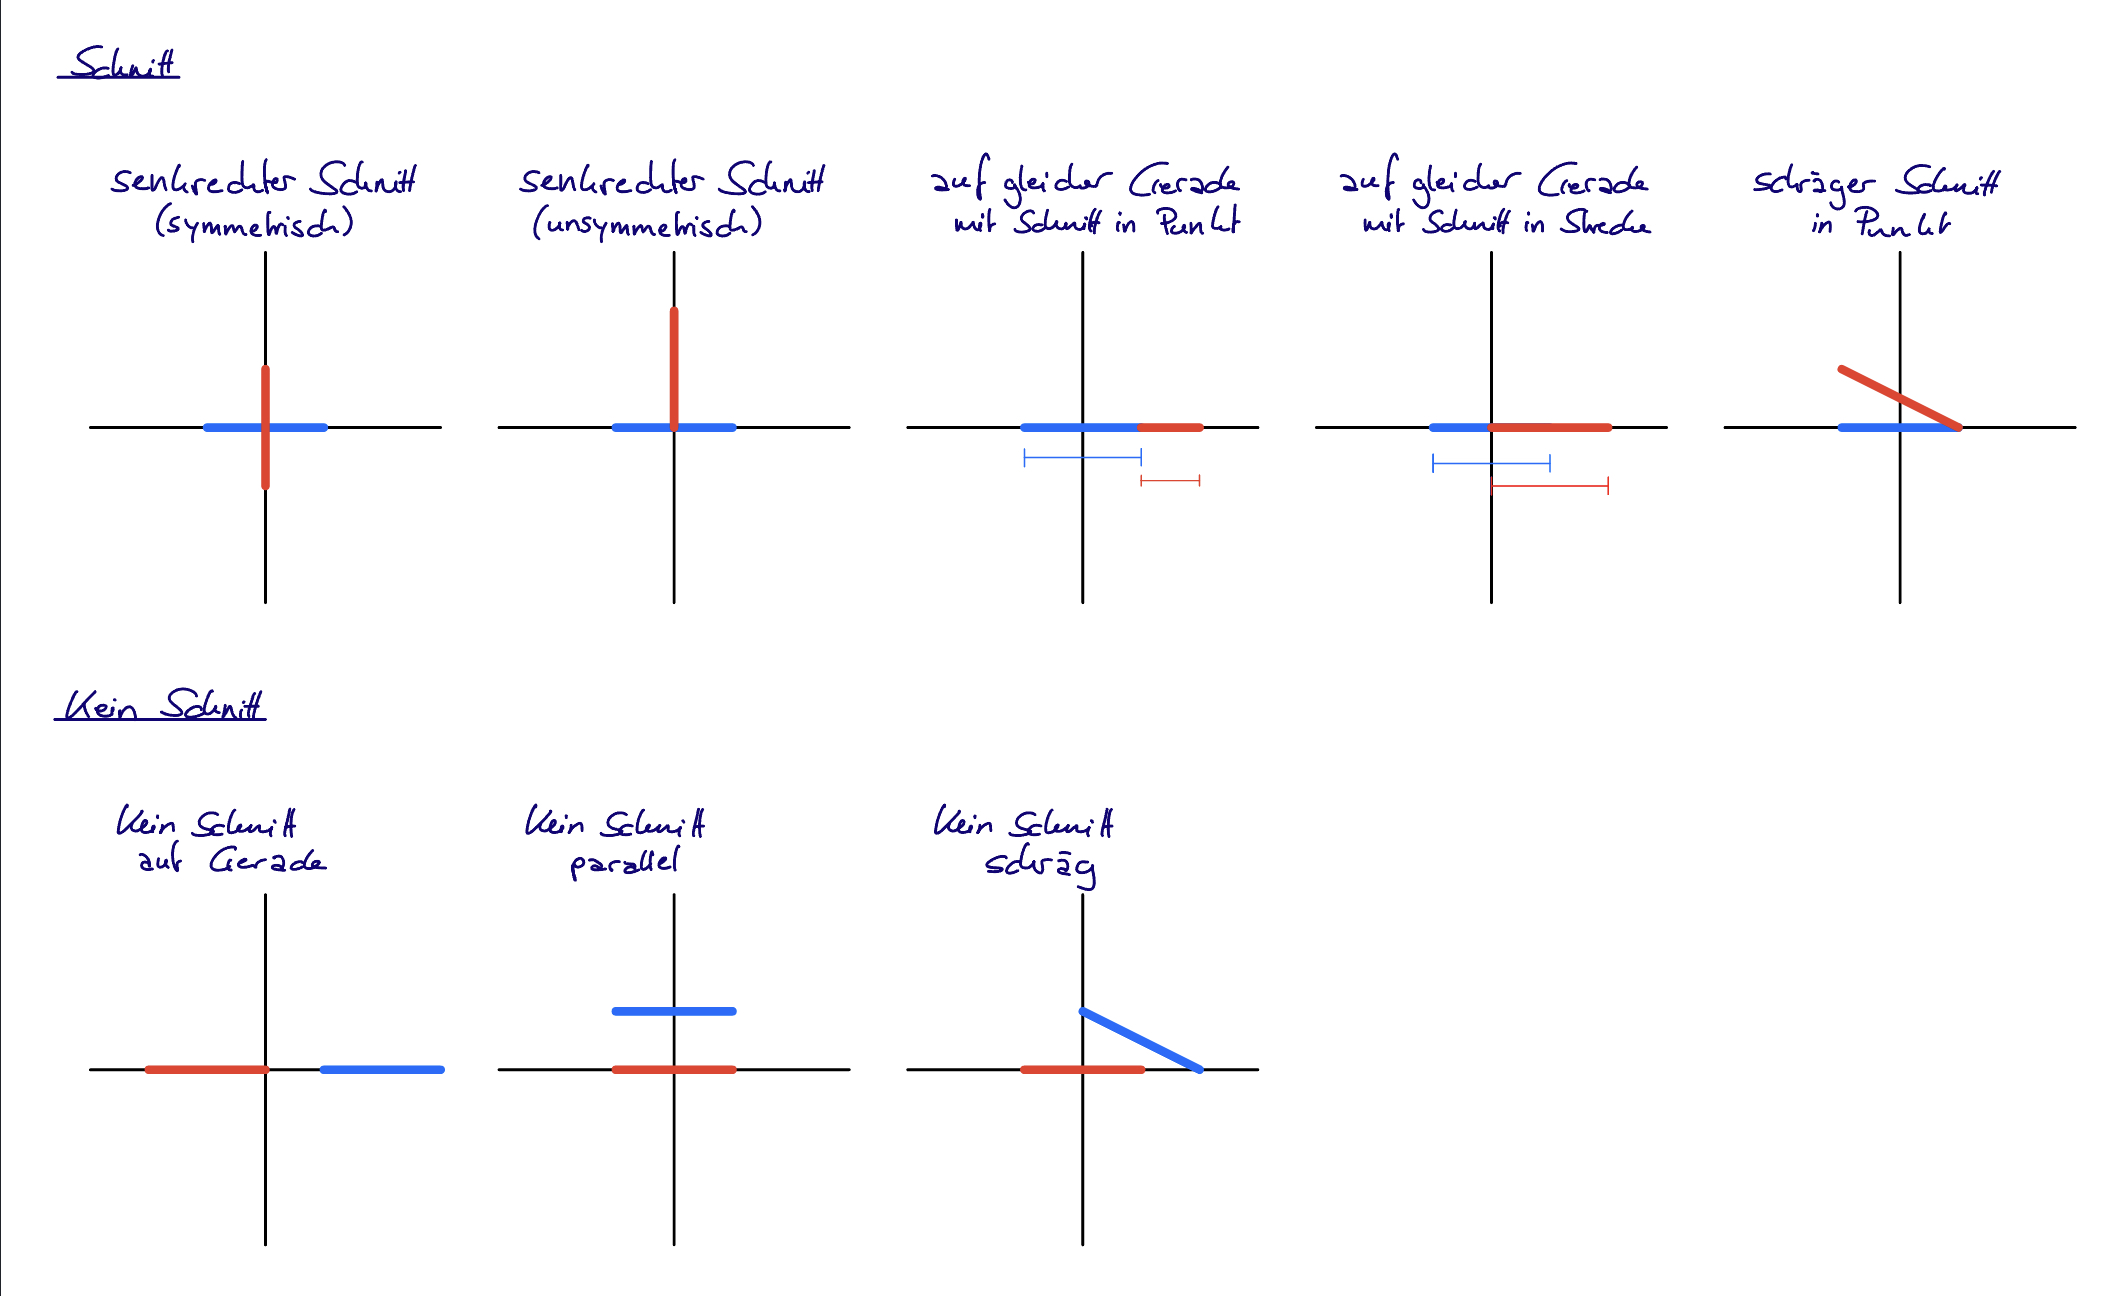
\includegraphics[scale=0.2]{Test_Vorlage.jpeg}
\end{figure}

Für jedes Streckenpaar ist zu berechnen, ob sie sich schneiden oder nicht.\\

\begin{lstlisting}[style=CStyle, caption={testing.cpp: Testen der Bibliotheksfunktionen},captionpos=b]
#include "p1_lib.h"

void print_result(line l1, line l2, bool b_soll){
    std::cout << std::boolalpha << "Soll: " << b_soll << ", Ist: " << line_intersect_check(l1, l2) << "\n";
}


int main(){

    // Verschiedene Schnitte

    // Strecken mit senkrechtem Schnitt (symmetrisch)
    // p1 = (0,1) nach p2 = (0,-1)
    // p1 = (1,0) nach p2 = (-1,0
    print_result(line{.p1.x = 0, .p1.y = 1, .p2.x = 0, .p2.y = -1}, line{.p1.x = 1, .p1.y = 0, .p2.x = -1, .p2.y = 0}, true);

    // Strecken mit senkrechtem Schnitt (unsymmetrisch)
    // p1 = (0,2) nach p2 = (0,0)
    // p1 = (1,0) nach p2 = (-1,0)
    print_result(line{.p1.x = 0, .p1.y = 2, .p2.x = 0, .p2.y = 0}, line{.p1.x = 1, .p1.y = 0, .p2.x = -1, .p2.y = 0}, true);
    
    // Strecken auf gleicher Gerade mit Schnitt in einem Punkt
    // p1 = (1,0) nach p2 = (2,0)
    // p1 = (1,0) nach p2 = (-1,0)
    print_result(line{.p1.x = 1, .p1.y = 0, .p2.x = 2, .p2.y = 0}, line{.p1.x = 1, .p1.y = 0, .p2.x = -1, .p2.y = 0}, true);

    // Strecken auf gleicher Gerade mit Schnitt in einer Strecke
    // p1 = (0,0) nach p2 = (2,0)
    // p1 = (1,0) nach p2 = (-1,0)
    print_result(line{.p1.x = 0, .p1.y = 0, .p2.x = 2, .p2.y = 0}, line{.p1.x = 1, .p1.y = 0, .p2.x = -1, .p2.y = 0}, true);

    // Strecken auf gleicher Gerade mit Schnitt in einer Strecke
    // p1 = (0,0) nach p2 = (2,0)
    // p1 = (1,0) nach p2 = (-1,0)
    print_result(line{.p1.x = 1, .p1.y = 0, .p2.x = -1, .p2.y = 1}, line{.p1.x = 1, .p1.y = 0, .p2.x = -1, .p2.y = 0}, true);


    // Verschiedene ohne Schnitt

    // Strecken ohne Schnitt auf Gerade
    // p1 = (-2,0) nach p2 = (0,0)
    // p1 = (1,0) nach p2 = (3,0)
    print_result(line{.p1.x = -2, .p1.y = 0, .p2.x = 0, .p2.y = 0}, line{.p1.x = 1, .p1.y = 0, .p2.x = 3, .p2.y = 0}, false);

    // Strecken ohne Schnitt parallel
    // p1 = (-2,0) nach p2 = (0,0)
    // p1 = (-2,1) nach p2 = (0,2)
    print_result(line{.p1.x = -2, .p1.y = 0, .p2.x = 0, .p2.y = 0}, line{.p1.x = -2, .p1.y = 1, .p2.x = 0, .p2.y = 2}, false);

    // Strecken ohne Schnitt schraeg
    // p1 = (-2,0) nach p2 = (0,0)
    // p1 = (0,1) nach p2 = (2,0)
    print_result(line{.p1.x = -2, .p1.y = 0, .p2.x = 0, .p2.y = 0}, line{.p1.x = 0, .p1.y = 1, .p2.x = 2, .p2.y = 0}, false);

    return 0;
}
\end{lstlisting}

\ \\~\\
Wie untenstehend gezeigt wird für alle Streckenpaare korrekt berechnet ob sie sich schneiden oder nicht.\\

\begin{lstlisting}[style=Terminal, caption={testing.cpp: Ausgabe Konsole},captionpos=b]
Soll: true, Ist: true
Soll: true, Ist: true
Soll: true, Ist: true
Soll: true, Ist: true
Soll: true, Ist: true
Soll: false, Ist: false
Soll: false, Ist: false
Soll: false, Ist: false    
\end{lstlisting}



\end{document}




